\section{Version Control}
\label{sec:VersionControl}

% Track changes in Word can cause many revisions, for example if remove space after paragraph is applied to a table then every cell will be a revision.
% Comparing git diff with current Word-based methods.
% Security and how you can self-host a git server.
% Log of changes - who made what change and when.
% Blobs are hashed. Can use signed commits to confirm what time commits were made.
% https://github.com/HenryGinn/Essays/tree/main/TheCaseForLaTeX

In this section I want to compare currently used version control methods for Word documents with what is possible with \LaTeX. One of the main powers of \LaTeX\ is that it is fully compatible with text-based version control software such as Git, the free and open source software used by almost all developers and software companies. Here we will not look at all the features of Git or how it works, but trust that it is more than powerful enough for the needs of WSP.

\subsection{Current Practice}

There are two main types of differences that someone may care about:

\begin{itemize}
	\item Changes in meaning such as ``Updated system description to comply with requirement xyz".
	\item All changes to the text and formatting.
\end{itemize}

On my current project we track the former in a table of changes and the latter with cross-through formatting and green highlighting. It may be the case that this project has a uniquely horrifying version control policy, but nonetheless it is worth highlighing the problems with it.

\begin{itemize}
	\item \textbf{Manually recording changes.} If someone forgets to record the change or incorrectly applies the formatting then the change is not properly tracked. As Git does this automatically it saves the need for the author to do it and also ensures it is always done correctly.
	\item \textbf{The document is harder to read.} The current version should not be polluted by the remnants of superseded parts. I regularly see paragraphs weaving in and out of superseded and non-superseded text which makes the current version hard to parse. It is not possible to easily see the document without the version control formatting either.
	\item \textbf{Updating revisions.} When a new revision is being prepared, the first task is to remove all text with cross-through formatting and remove all green highlight. This is a manual task that should not exist. As before, this process is also error prone - consider figure~\ref{fig:4Strikethrough} where it is almost impossible to see the difference between a four that has been removed from the document and one that has been added. Figure~\ref{fig:UnclearStrikethrough} has a single row that has been removed that could easily be missed when preparing the next revision.
	\item \textbf{Formatting.} Formatting in Word is often inherent to the subject of the formatting or is given by invisible characters\footnote{For example, the formatting of a bullet point or paragraph number is given by an invisible formatting character at the end of the clause and I have seen multiple people confused as to why they cannot clear highlighting from a previous revision.} so cannot be tracked by this method. Other changes in formatting such as the structure of a table can only be recorded by duplicating the whole table and applying cross-through formatting.
	\item \textbf{Confusion between types of change.} There is no distinction between the two types of changes making for useless tables of changes. I have seen sections completely rewritten with the description ``Text revised" and the tense of a single unimportant word changed where the letters that were added and removed were stated. Both of these examples followed the version control policy exactly.
\end{itemize}

\begin{figure}[!htb]
	% Store largest image in a box
	\savebox{\imagebox}{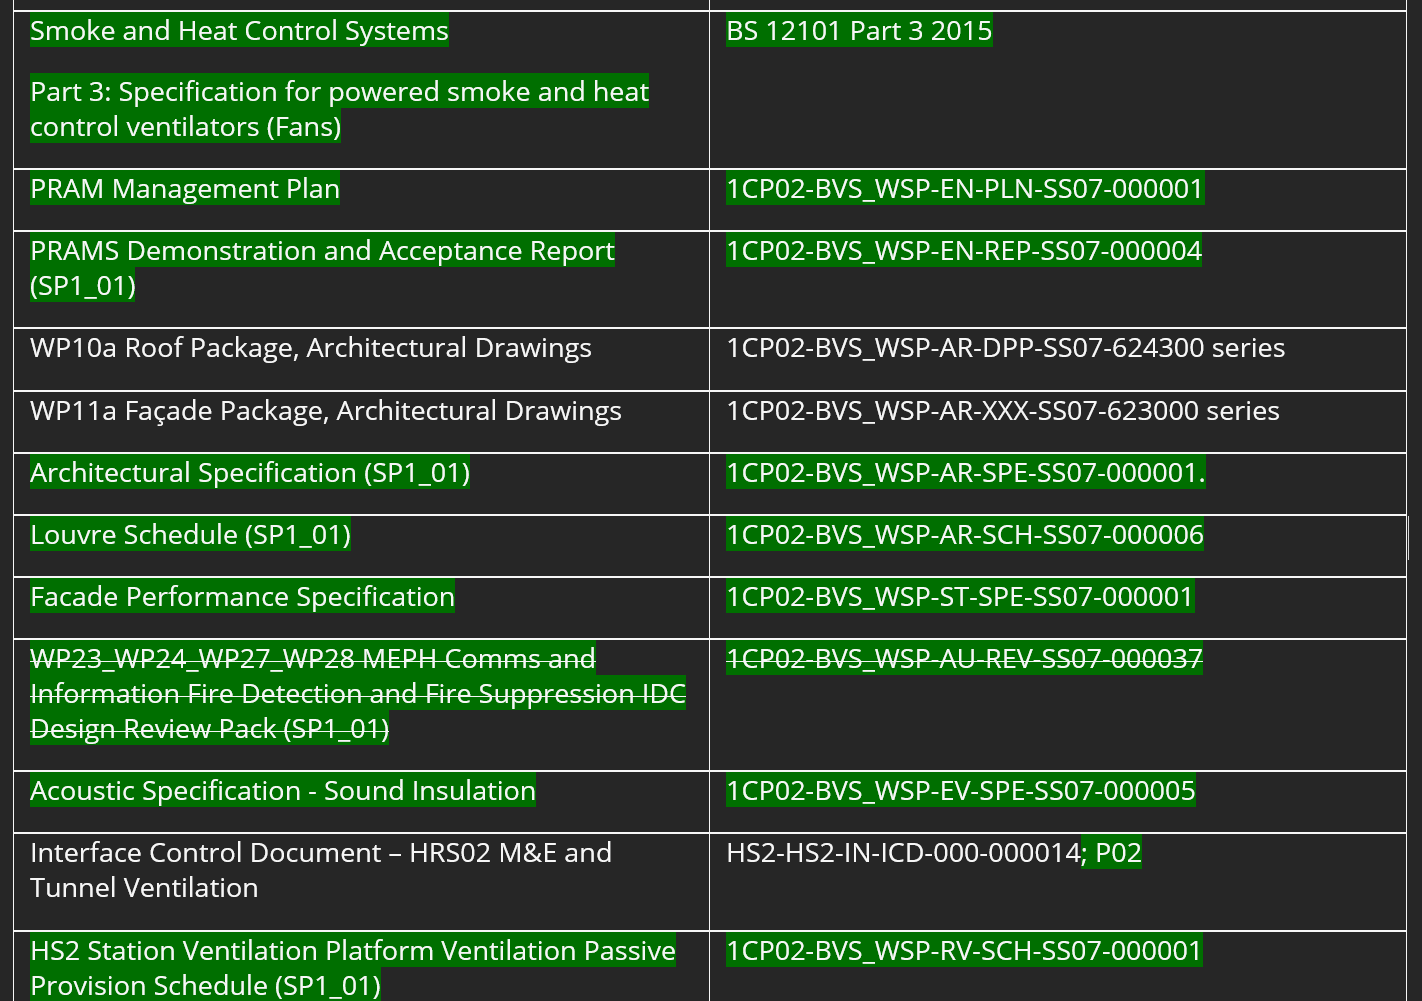
\includegraphics[width=0.75\textwidth]{Figures/ExampleOfPoorVersionControl.png}}
	\begin{subfigure}[t]{0.2\textwidth}
		\centering\raisebox{\dimexpr0.5\ht\imagebox-0.5\height}{% Raise smaller image into place
			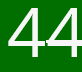
\includegraphics[width=\textwidth]{Figures/StrikethroughFour.png}}
			\caption{Strike-through comparison}
			\label{fig:4Strikethrough}
	\end{subfigure}
	\hfill
	\begin{subfigure}[t]{0.75\textwidth}
		\centering\usebox{\imagebox}% Place largest image
		\caption{Current version control example}
		\label{fig:UnclearStrikethrough}
	\end{subfigure}
	\caption{Examples of a current method of version control for Word documents.}
	\label{fig:WordVersionControl}
\end{figure}


\subsection{Resolution with \LaTeX\ and Git}

Let us see how an approach with \LaTeX\ and git avoids these problems. Before we look into how Git can avoid these issues we must first have some understanding of Git.

In short, after some changes are made the author creates something called a ``commit" which is a snapshot of the project at that point in time\footnote{Git does not store only the changes and it also does not create a copy of the whole project. It works in a clever way that is beyond the scope of this essay that means the total amount of stored data is small.}, and then this commit can be sent to a shared repository. \href{https://www.youtube.com/watch?v=e9lnsKot_SQ}{\underline{This video}} gives a simple explanation of the Git workflow for those wanting to know more.

The difference between any two commits can be produced on command is seen in figure~\ref{fig:ExampleOfDiff}.

\begin{figure}[!htb]
	\centering
	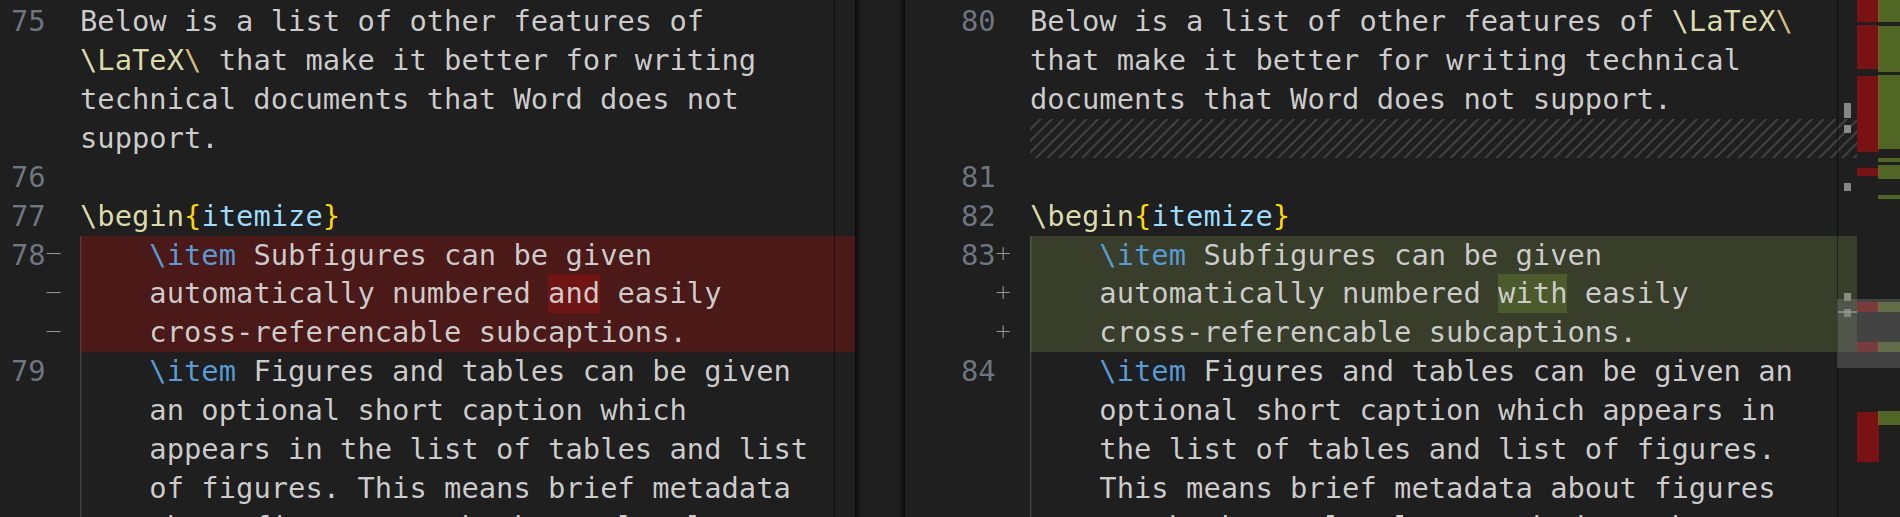
\includegraphics[width=\textwidth]{Figures/ExampleOfDiff2.png}
	\caption{An example of the difference between two files.}
	\label{fig:ExampleOfDiff}
\end{figure}

\LaTeX\ is also better for version control. As it is all text-based it can be used with version control software like Git, which gives tracability, control over branches, and easy computation of differences between versions. This also tracks any formatting changes that cannot be handled by the template such as the shape of a table.